\documentclass[paper=a4, fontsize=12pt]{scrartcl}
\usepackage{graphicx}
\usepackage[protrusion=true,expansion=true]{microtype}
\usepackage{amsmath,amsfonts,amsthm}
\usepackage{fourier}
\usepackage[utf8]{inputenc}
\usepackage{amsmath}
\usepackage{amsfonts}
\usepackage{amssymb}
\usepackage[OT4]{fontenc}
\usepackage[polish]{babel}
\usepackage{epstopdf}
\usepackage{fancyhdr}
\usepackage{hyperref}
\pagestyle{fancyplain}
\fancyhead{}	
\renewcommand{\headrulewidth}{1pt}
\renewcommand{\footrulewidth}{1pt}
\textheight = 700pt
\textwidth = 500pt
\hoffset =-30pt
\begin{document}
\begin{flushright}
05.05.2016 r.\\
dr Robert Bryl
\end{flushright}Paweł Grabiński\\
Rok 3, Fizyka teoretyczna\\[0.5cm]
{\huge \bf Praca wyjścia}
\section{Wyniki}
Praca wyjścia uzyskana metodą Richardsona to $W=4.95\pm0.22\:\mathrm{eV}$.\\
Praca wyjścia uzyskana metodą Davissona to $W=1.65\pm0.47\:\mathrm{eV}$.
\section{Tabela pomiarowa}

\subsection{Metoda Davissona}

\begin{table}[h!]
	\begin{tabular}{|l|l|l|l|}
		\hline
		$I_\mathrm{ż}\:[\mathrm{mA}]$ & $R\:[\mathrm{k\Omega}]$ & $I_a\:[\mathrm{mA}]$ & $\Delta I_\mathrm{ż}\:[\mathrm{mA}]$ \\ \hline
		24.98 & 11   & 5.358 & 2.339 \\ \hline
		23.97 & 10.6 & 5.142 & 2.258 \\ \hline
		23.01 & 10.3 & 4.819 & 2.099 \\ \hline
		21.96 & 9.9  & 4.431 & 1.945 \\ \hline
		20.97 & 9.5  & 4.006 & 1.754 \\ \hline
		19.87 & 9.1  & 3.503 & 1.525 \\ \hline
		19.02 & 8.6  & 2.958 & 1.226 \\ \hline
		18.06 & 8.34 & 2.348 & 0.991 \\ \hline
		17.05 & 7.91 & 1.703 & 0.680 \\ \hline
		16.01 & 7.46 & 1.035 & 0.515 \\ \hline
		14.99 & 7.02 & 0.497 & 0.263 \\ \hline
		13.96 & 6.43 & 0.144 & 0.394 \\ \hline
		13.02 & 6.05 & -     & -     \\ \hline
		12.06 & 5.55 & -     & -     \\ \hline
		11.04 & 5.04 & -     & -     \\ \hline
		10.02 & 4.55 & -     & -     \\ \hline
		9.01  & 4.12 & -     & -     \\ \hline
		7.99  & 3.8  & -     & -     \\ \hline
		7.03  & 3.55 & -     & -     \\ \hline
		6.09  & 3.37 & -     & -     \\ \hline
		5.03  & 3.21 & -     & -     \\ \hline
		4.01  & 3.1  & -     & -     \\ \hline
		2.94  & 3.01 & -     & -     \\ \hline
		2.02  & 3.01 & -     & -     \\ \hline
		1.05  & 3.01 & -     & -     \\ \hline
	\end{tabular}
\end{table}\clearpage
\subsection{Methoda Richardsona}
\begin{table}[h!]
	\begin{tabular}{|l|l|l|l|l|l|l|l|l|l|l|}
		\hline
		$I_\mathrm{ż}\:[\mathrm{mA}]$ & 1199 & 1249 & 1299 & 1350 & 1403 & 1452 & 1503 & 1549  & 1600  & 1649 \\ \hline
		$I_a\:[\mathrm{mA}]$ & 1.3  & 2.7  & 5.3  & 10.5 & 20.4 & 37.0 & 66.6 & 108.8 & 187.6 & 300  \\ \hline
		$T_\uparrow\:[\mathrm{\:^\circ C}]$ & 1020 & 1040 & 1060 & 1100 & 1100 & 1120 & 1140 & 1160  & 1180  & 1200 \\ \hline
		$T_\downarrow\:[\mathrm{\:^\circ C}]$ & 1040 & 1060 & 1060 & 1100 & 1120 & 1120 & 1140 & 1160  & 1180  & 1220 \\ \hline
	\end{tabular}
\end{table}
\section{Opis teoretyczny}
\subsection{Teoria ciała stałego}
\subsubsection{Model pasmowy}
Pasmowy model ciała stałego jest to teoria opierająca wyjaśnienie własności ciał stałych (metali półprzewodników i dielektryków) na założeniu, że energie elektronów wchodzących w ich skład nie są dowolne, lecz należą do ściśle określonych zakresów, zwanych dozwolonymi pasmami energetycznymi. Pasma te są rozdzielone wzbronionymi pasmami energetycznymi, tzn. zakresami wartości energii, których nie może mieć żaden elektron znajdujący się w ciele stałym. Model prawieswobodnych elektronów w periodycznym polu potencjale umożliwia zrozumienie przewodnictwa elektrycznego w ciałach stałych. W wyniku powstawania cząstek oraz kryształów, poziomy energetyczne pojedynczego atomu zmieniają się wskutek nakładania się rozkładów elektronowych na siebie. Rozważymy dla przykładu układ $N$ atomów wodoru. Jeżeli zbliżymy je do siebie, poziomy energetyczne ulegają rozszczepieniu zgodnie z zakazem Pauliego - każdy z poziomów musi ulec degeneracji na $N$ stanów.\\
\begin{figure}[h!]
\centering
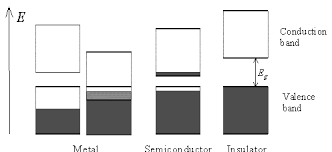
\includegraphics[width=0.7\linewidth]{pasm}
\caption{Model obsadzania elektronami dozwolonych pasm energetycznych w izolatorze, metalu, i dwóch półprzewodnikach. Pionowe rozmiary prostokątów przedstawiają dozwolone obszary energii, pola zacieniowane oznaczają obszary wypełnione elektronami.}
\label{fig:pasm}
\end{figure}\\
W ciałach krystalicznych możemy przyjąć ze względu na bardzo dużą liczbę atomów w krysztale, że stopień degneracji dąży do nieskończoności. Dzięki temu powstają pasma o praktycznie ciągłych zakresach energii. Elektrony mogą przyjmować jedną z wielu zbliżonych do siebie energii tworzących pasmo energetyczne. Elektrony zaczną przenikać do sąsiednich atomów w wyniku tunelowania przez obszary, w których energia potencjalna elektronu jest wyższa niż energia całkowita. Dzięki tunelowaniu elektrony zyskują swobodę poruszania się po całym krysztale - tworzą gaz elektronowy.\\

Pasma energetyczne pomiędzy pasmami dozwolonymi nazywamy przerwami energetycznymi. Jeżeli dozwolone pasma energetyczne są całkowicie wypełnione albo puste, to wówczas elektrony nie mogą poruszać się w polu elektrycznym i kryształ zachowuje się jak izolator. Jeżeli jedno lub więcej pasm jest częściowo zapełnione, to kryształ zachowuje się  jak metal. Jeżeli wszystkie pasma są całkowicie zapełnione z wyjątkiem jednego lub dwóch 
pasm, które są tylko nieznacznie zapełnione lub prawie puste, to wówczas kryształ jest półprzewodnikiem. 
\subsection{Rozkład Fermiego-Diraca}
Rozkład Fermiego-Diraca opisuje stany obsadzone przez fermiony w układzie. Jak wiemy elektorny są fermionami. Rozkład ten daje nam prawdopodobieństo obsadzenia kolejnych stanów energetycznych przy danej temperaturze.
\begin{align*}
	f(\varepsilon,T)=\frac{1}{\exp\left(\frac{\varepsilon-\varepsilon_F}{k_bT}\right)+1}
\end{align*}
W temperaturze $0\:\mathrm{K}$ obsadzone są tylko stany poniżej stanu Fermiego.
\begin{figure}[h!]
\centering
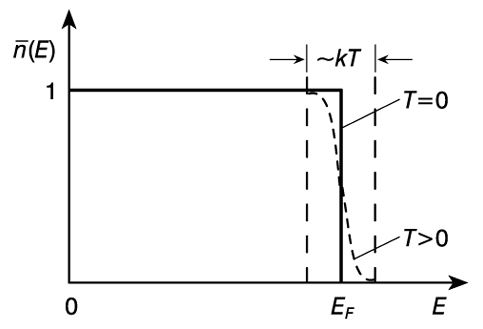
\includegraphics[width=0.5\linewidth]{d82i2792}
\label{fig:d82i2792}
\end{figure}

\subsubsection{Praca wyjścia}
Elektrony w metalach są łatwo separowalne od atomów, które stają się w jonami dodatnimi. Tworzą one regularną sieć krystaliczną metalu. Oddziaływania ze strony jonów sieci krystalicznej na elektrony znoszą się wzajemnie. Uzyskujemy obraz swobodnych elektronów. Mówimy o gazie elektronowym w metalu. Pomimo swobody pomiędzy jonami sieci krystalicznej metalu, elektorny nie mogą go opuścić. Na powierzchni metalu oddzialywanie te nie znoszą się. Możemy obserwować siłę obrazową działającą na elektron znajdujący się poza objętością metalu. By pokonać te oddziaływania elektron musi wykonać pewną pracę - pracę wyjścia. Oddziaływania te możemy opisać jako barierę potencjału.
\begin{figure}[h!]
\centering
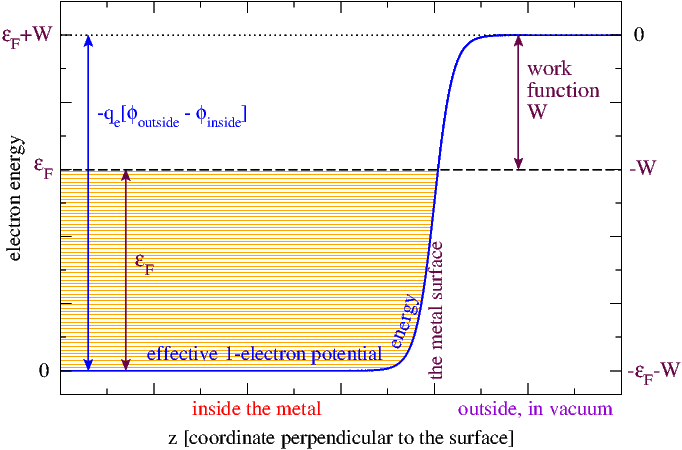
\includegraphics[width=0.7\linewidth]{FermiMetal}
\caption{Energia potencjalna elektronu w pobliżu powierzchni metalu. Po lewej mamy zaznaczone, zgodnie z ideą energii Fermiego, poziomy energetyczne elektronów przewodnictwa w temperaturze zerowej - mamy obsadzone wszystkie poziomy energetyczny poniżej energii Fermiego.}
\label{fig:FermiMetal}
\end{figure}\\
Jeżeli elektronom dostarczymy dodatkowej energii, to zajmą one wyższe poziomy energetyczne niż poziom Fermiego. Niektóre z nich mogą opuścić metal. Energia realizowana w trakcie opuszczania metalu przez elektorn nazywana jest pracą wyjścia i wyraża się jak:
\begin{align*}
W=e\phi=e(\phi_{outside}-\phi_{inside})
\end{align*}
Gdzie $\phi$ nazywamy potencjałem wyjścia. Wartość pracy wyjścia zależy od rodzaju materiału i dla czystych metali zawiera się w granicach od ok. $1.5$ do kilku elektronowoltów. Zależy ona również do stanu powierzchni metalu. Zanieczyszczenie powierzchni przez inne substancje lub gazy absorbowane mogą bądź zmniejszyć bądź zwiększyć pracę wyjścia. Substancje o małej pracy wyjścia mają właściwości obniżania bariery potencjału, a więc zmniejszają pracę wyjścia z elektronów metalu stanowiącego ich podłoże. Dzięki tym właściwościom substancje te są używane w lampach elektronowych do wyrobu tzw. katod aktywowanych.
\subsubsection{Potencjał kontaktowy}
Każdy metal możemy opisać pewnym ustalonym poziomem Fermiego. Jeśli zetkniemy powierzchnie dwóch metali, to zobserwujemy \textbf{kontaktową różnicę potencjałów}, który wynika z różnicy poziomów Fermiego. Elektrony z metalu o wyższej energii Fermiego (mniejszej pracy wyjścia), mogą tunelować przez barierę potencjału między powierzchniami metali do metalu o niższej energii Fermiego (większej pracy wyjścia). Układ będzie dążyć do minimalizacji energii. Dojdzie do wyrównania poziomów Fermiego. Pomiędzy powierzchniami wytowrzy się pole elektryczne spowodowane przesunięciem ładunku z jednego metalu do drugiego. Pole to będzie stanowiło barierę energetyczną dla kolejnych elektronów. Otrzymamy układ w równowadze termodynamicznej.
\subsection{Teoria diody}
Emisję elektronową wykorzystują lampy elektronowe zwane potocznie diodą. Dioda składa się z katody stanowiącej źródło elektronów i anodę, do której pod wpływem przyłączonego napięcia docierają emitowane elektrony. Ruch elektronów w lampie powoduje w obwodzie anodowym przepływ prądu anodowego. Natężenie tego prądu jest zależne od napięcia anody.  
\begin{figure}
\centering
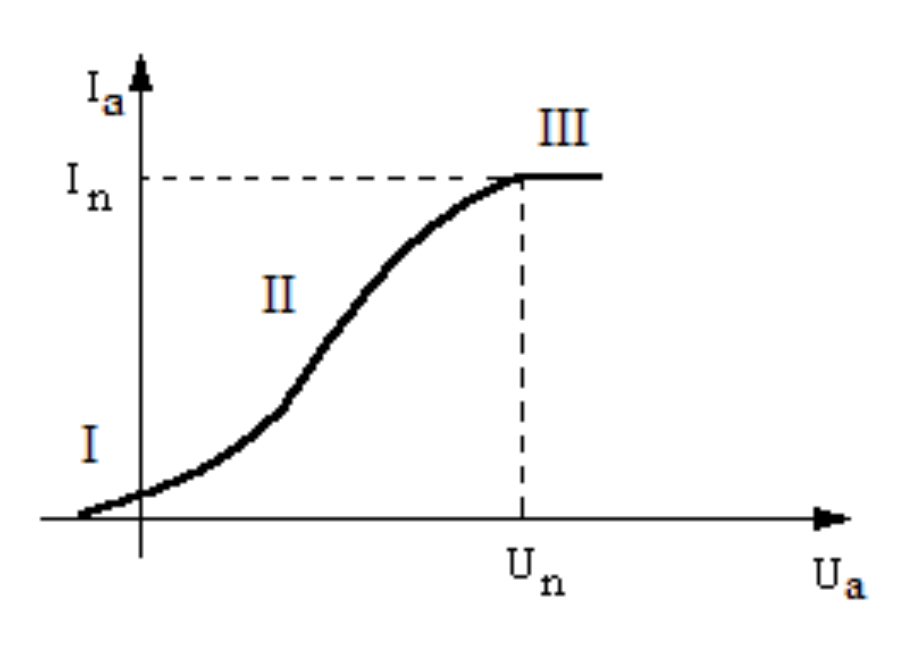
\includegraphics[width=0.4\linewidth]{dioda}
\caption{Charakterystyka diody próżniowej w stałej temperaturze.}
\label{fig:dioda}
\end{figure}\\
Charakterystykę tę możemy podzielić na trzy obszary w zależności od zachodzących w nich zjawisk.
\subsubsection{Zakres I - prądu początkowego}
	
	Obejmuje ujemne napięcia anody. Prąd początkowy powstaje wskutek docierania do anody tylko najbardziej energetycznych elektronów, które są w stanie pokonać potencjał. Prąd anody jest zwykle niewielki, szybko malejący w miarę zmniejszana napięcia anody.
\subsubsection{Zakres II - ładunku przestrzennego}
	
	Obejmuje dodatnie napięcia mniejsze od napięcia nasycenia. Występuje tu hamowania elektronów w polu innych elektronów, w ten sposób powstaje chmura ładunku pomiędzy katodą i anodą. 
\subsubsection{Zakres III - nasycenia}
	
	Napięcie powyżej napięcia nasycenia. Jeżeli do anody przyłożymy odpowiednio duże napięcie, spowodujemy przepływ elektronów otaczających katodę do anody, co powoduje zmniejszenie potencjału hamującego i w rezultacie wzrost prądu anody. Jeżeli przyłożymy wystarczająco duże napięcie zwane napięciem nasycenia, prąd anody osiągnie wartość równą prądowi emisyjnemu katody. Napięcie większe od napięcia nasycenia nie może spowodować wzrostu prądu anody, bowiem już przy napięciu nasycenia wszystkie elektrony emitowane przez katodę brały udział w przepływie prądu.
\subsubsection{Katody tlenkowe}
Katody tlenkowe mają postać rdzenia metalowego (najczęściej niklowego), pokrytego warstwą tlenków metali ziem alkalicznych (baru, strontu, wapnia). Powoduje to zmniejszeni pracy wyjścia elektronu z katody, a co za tym idzie wzrost natężenia prądu anody. W lampach elektronowych z katodą tlenkową nie osiąga się prądu nasycenia. Przy podwyższaniu napięcia anody natężenie prądu szybko wzrasta i przy pewnej krytycznej wartości I katoda ulega zniszczeniu. Katody te odznaczają się bardzo dobrymi właściwościami i dlatego są stosowane w znacznej większości lamp elektronowych.
\subsection{Układ Davissona}
Pracę wyjścia elektronu z metalu można wyznaczyć między innymi metodą Davissona. Metoda ta polega na kompensacji ochładzania katody. W zjawisku emisji termoelektronowej wykonanie pracy wyjścia i nadanie prędkości początkowej emitowanym elektronom odbywa się kosztem energii cieplnej katody. Gdy elektrony nie są odprowadzane z przestrzeni w pobliżu katody, wówczas tworzy się tam ładunek przestrzenny, powodujący ustalenie się równowagi dynamicznej pomiędzy elektronami wychodzącymi z katody i powracającymi do niej. Wytwarzając odpowiednie pole elektryczne można wszystkie elektrony wylatujące z rozżarzonej katody oddalić od niej. W takim razie temperatura katody obniży się (wskutek straty energii na emisję). Chcąc ją podwyższyć do wartości poprzedniej, należy zwiększyć moc żarzenia o dP. Moc żarzenia możemy przedstawić jako iloczyn oporu włókna katody oraz kwadratu prądu żarzenia:
\begin{align*}
P=I_\mathrm{ż}^2R
\end{align*}
Zwiększając moc o $dP$:
\begin{align*}
P+dP=(I_\mathrm{ż}+dI_\mathrm{ż})^2R=R(I_\mathrm{ż}^2+2I_\mathrm{ż}dI_\mathrm{ż}+dI_\mathrm{ż}^2)
\end{align*}
Czyli przyrost mocy możemy, przy założeniu $dI_\mathrm{ż}\approx 0$, wyrazić jako:
\begin{align*}
dP=P+dP-P=R(I_\mathrm{ż}^2+2I_\mathrm{ż}dI_\mathrm{ż}+dI_\mathrm{ż}^2)-I_\mathrm{ż}^2R=R(2I_\mathrm{ż}dI_\mathrm{ż}+dI_\mathrm{ż}^2)\approx2I_\mathrm{ż}dI_\mathrm{ż}R
\end{align*}
Z rozważań statystycznych wiemy, że średnią energię kinetyczną elektornu możemy wyrazić jako $2k_bT$. Biorąc pod uwagę, że elektorny są wypromieniowywane z ciała o temperaturze $T$, a powracają przez układ o temperaturze $T_0$, to możemy wyrazić pracę emisji jako:
\begin{align*}
W_{emi}=W+2k_b(T-T_0)
\end{align*}
Gdzie $W$ to szukana przez nas praca wyjścia. Całkowity przyrost mocy jest proporcjonalny do liczby emitowanych elektronów które możemy wyrazić jako $N=\frac{I_a}{e}$. W takim razie:
\begin{align*}
dP=\frac{I_a}{e}W_{emi}=\frac{I_a}{e}(W+2k_b(T-T_0))
\end{align*}
Zestawiając to z poprzednim wynikiem na $dP$ , przekształcamy do postaci wyrażenia na pracę wyjścia $W$:
\begin{align*}
2I_\mathrm{ż}dI_\mathrm{ż}R=\frac{I_a}{e}(W+2k_b(T-T_0))\\
W=\frac{2eI_\mathrm{ż}dI_\mathrm{ż}R}{I_a}-2k_b(T-T_0)
\end{align*}
Doświadczalnie możemy wyznaczyć wszystkie potrzebne parametry.
\subsection{Pirometr}
Pirometr jest urzadzeniem służącym do pomiaru temperatury ciał o wysokich energiach. Zbudowany jest z układu optycznego obiektyw-filtr-okular, a pomiędzy obiektywem i filtrem umieszczone jest żarzące się włókno wolframowe. Pomiar polega na porównywaniu natężenia promieniowania włókna i obserwowanego obiektu.
By pomiar ten był możliwy należy wcześniej wyskoalować przyrząd na wzorcowym ciele doskonale czarnym.
\subsection{Metoda Richardsona}
Korzystając z prawa Richardsona, możemy dojść równania zawierającego mierzone przez nas wielkości:
\begin{align*}
J_N=aT^2\exp(-\frac{W}{k_bT})\qquad \|\cdot T^{-2}\\
\frac{J_N}{T^{-2}}=a\exp(-\frac{W}{k_bT})\qquad \|\ln(\#)\\
\ln(\frac{J_N}{T^{-2}})=\ln a-\frac{W}{k_bT}
\end{align*}
Sporządając wykres $\ln(\frac{J_N}{T^{-2}})=f(\frac{1}{k_bT})$ otrzymamy linię prostą, której współczynnik kierunkowy będzie równy pracy wyjścia $W$.\clearpage
\section{Analiza pomiarów}
\subsection{Metoda Richardsona}
\subsubsection{Opis pomiarów}
W metodzie tej układ pomiarowy składa sie z diody i pirometru. Do katody doprowadzamy prąd o zadanym natężeniu żarzenia, na anodzie mierzy natężenie prądu anodowego. Za pomocą pirometru mierzymy temperaturę katody.\\

W naszych pomiarach dokonywaliśmy pomiaru temperatury katody oraz natężenia prądu katodowego w zależności od natężenia pradu żarzenia w zakresie od $1650-1200\:\mathrm{mA}$.\\
Pomiarów temperatury dokonywaliśmy dwa razy. Raz zwiększając nateżęnie włókna w pirometrze, a raz je zmniejszając.
\subsubsection{Temperatura, a prąd żarzenia}
\begin{figure}[h!]
\centering
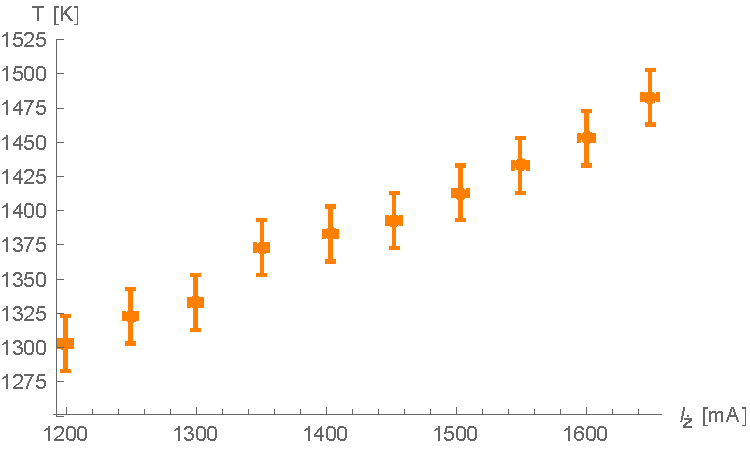
\includegraphics[width=0.8\linewidth]{tiz}
\caption{Zależność temperatury od prądu żarzenia. \newline Niepewność temperatury wzięta jako szerokość podziałki $20\:^\circ C$. Niepewność prądu żarzenia wyznaczona jako $\Delta I_\mathrm{ż}=0.3\%\cdot I_\mathrm{ż}+0.1\%dI$, gdzie $dI=1000\:\mathrm{mA}$ to zakres pomiarowy.}
\label{fig:tiz}
\end{figure}
\subsubsection{Prosta Richardsona}
Dalej możemy zgodnie z przyjętą metodą przez nas wykreślić zależność $\ln(\frac{J_N}{T^{-2}})=f(\frac{1}{k_bT})$. \\Korzystamy z zależności $I=j\cdot d^2$, a stałą Boltzmana przyjmujemy $k_B=1.380658 \cdot10^{-23}\:\mathrm{\frac{J}{K}}$.
\clearpage
\begin{figure}[h!]
\centering
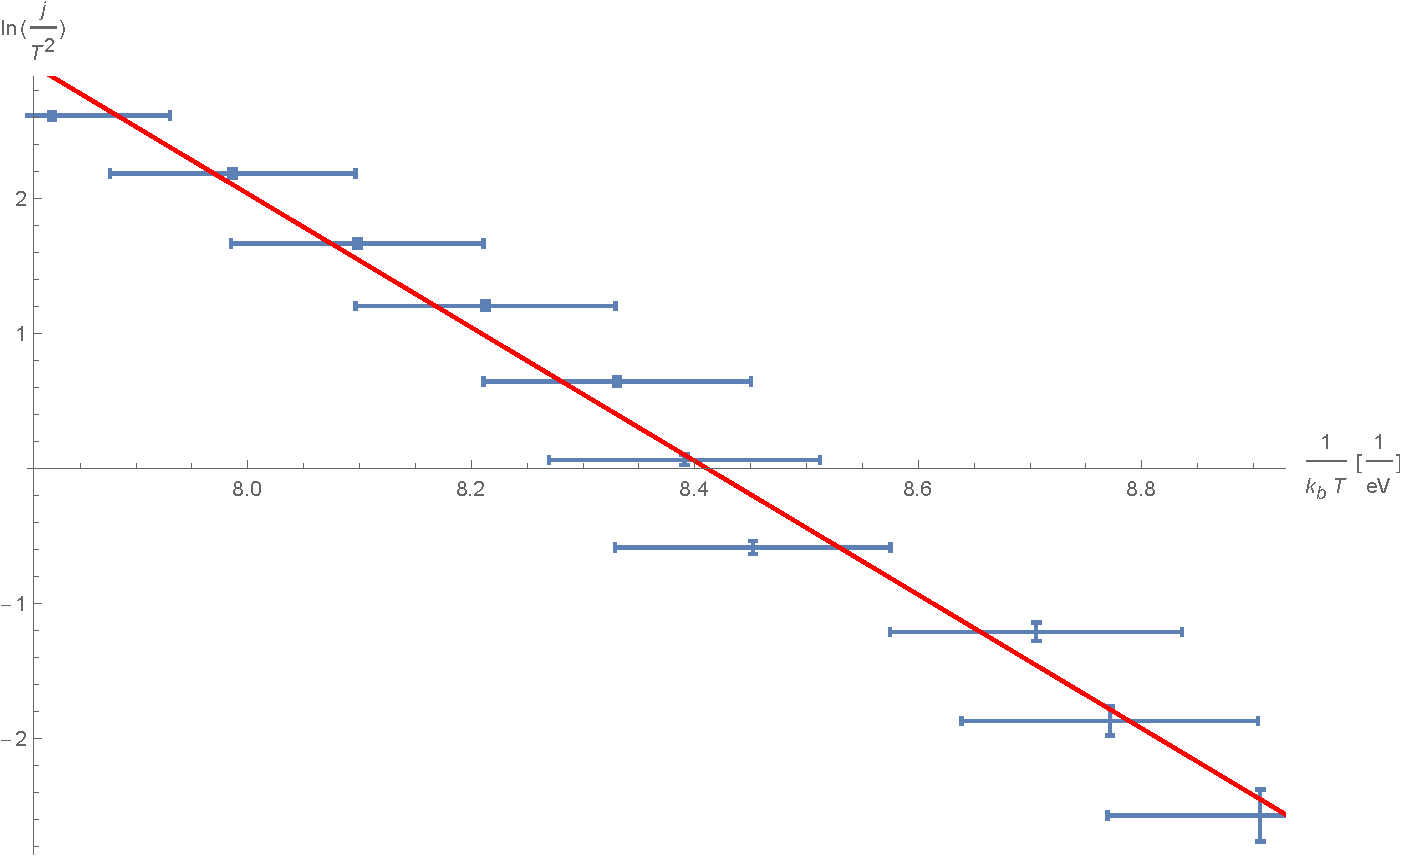
\includegraphics[width=0.8\linewidth]{prrich}
\caption{Możemy dopasować do danych linię prostą, której współczynnik nachylenie jest co do wartości równy pracy wyjścia. }
\label{fig:prrich}
\end{figure}
Niepewności tych wielkości wyznaczyliśmy z różniczki zupełnej.
\begin{align*}
\Delta(\ln\left(\frac{I_a}{d^2T^2}\right))=\left|\frac{\partial\ln\left(\frac{I_a}{d^2T^2}\right)}{\partial I_a}\right|\Delta I_a +
\left|\frac{\partial\ln\left(\frac{I_a}{d^2T^2}\right)}{\partial T}\right|\Delta T=
=\frac{\Delta I_a}{I_a}+\frac{2 \Delta T}{T}\\
\Delta \left(\frac{1}{k_bT}\right)=\left|\frac{\partial\left(\frac{1}{k_bT}\right)}{\partial T}\right|\Delta T=
\frac{\Delta T}{k_b T^2}
\end{align*}
Natomiast niepewność współczynnika prostej - pracy wyjścia uzyskaliśmy z liniowego modelu pakietu Mathematica.
\subsubsection{Wynik}
Uzyskana praca wyjścia dla włókna katody wolframowej to $W=4.95\pm0.22\:\mathrm{eV}$.
\subsection{Metoda Davissona}
\subsubsection{Opór włókna}
Ponieważ mostek był zrówoważony, to możemy wyrazić opór włókna:
\begin{align*}
R=\frac{R_1}{R_4}R_3=10^{-2}R_3
\end{align*}
Biorąc pod uwagę, że oporniki w układzie miały odpowiednio charakterystyki $R_1=100\:\mathrm{\Omega}$ i $R_4=10\:\mathrm{k\Omega}$.
\subsubsection{Temperatura}
Temperaturę mierzymy poprzez pomiar rezystancji.\\
Na początek wyzaczamy opór w temperaturze pokojowej.
\begin{figure}
\centering
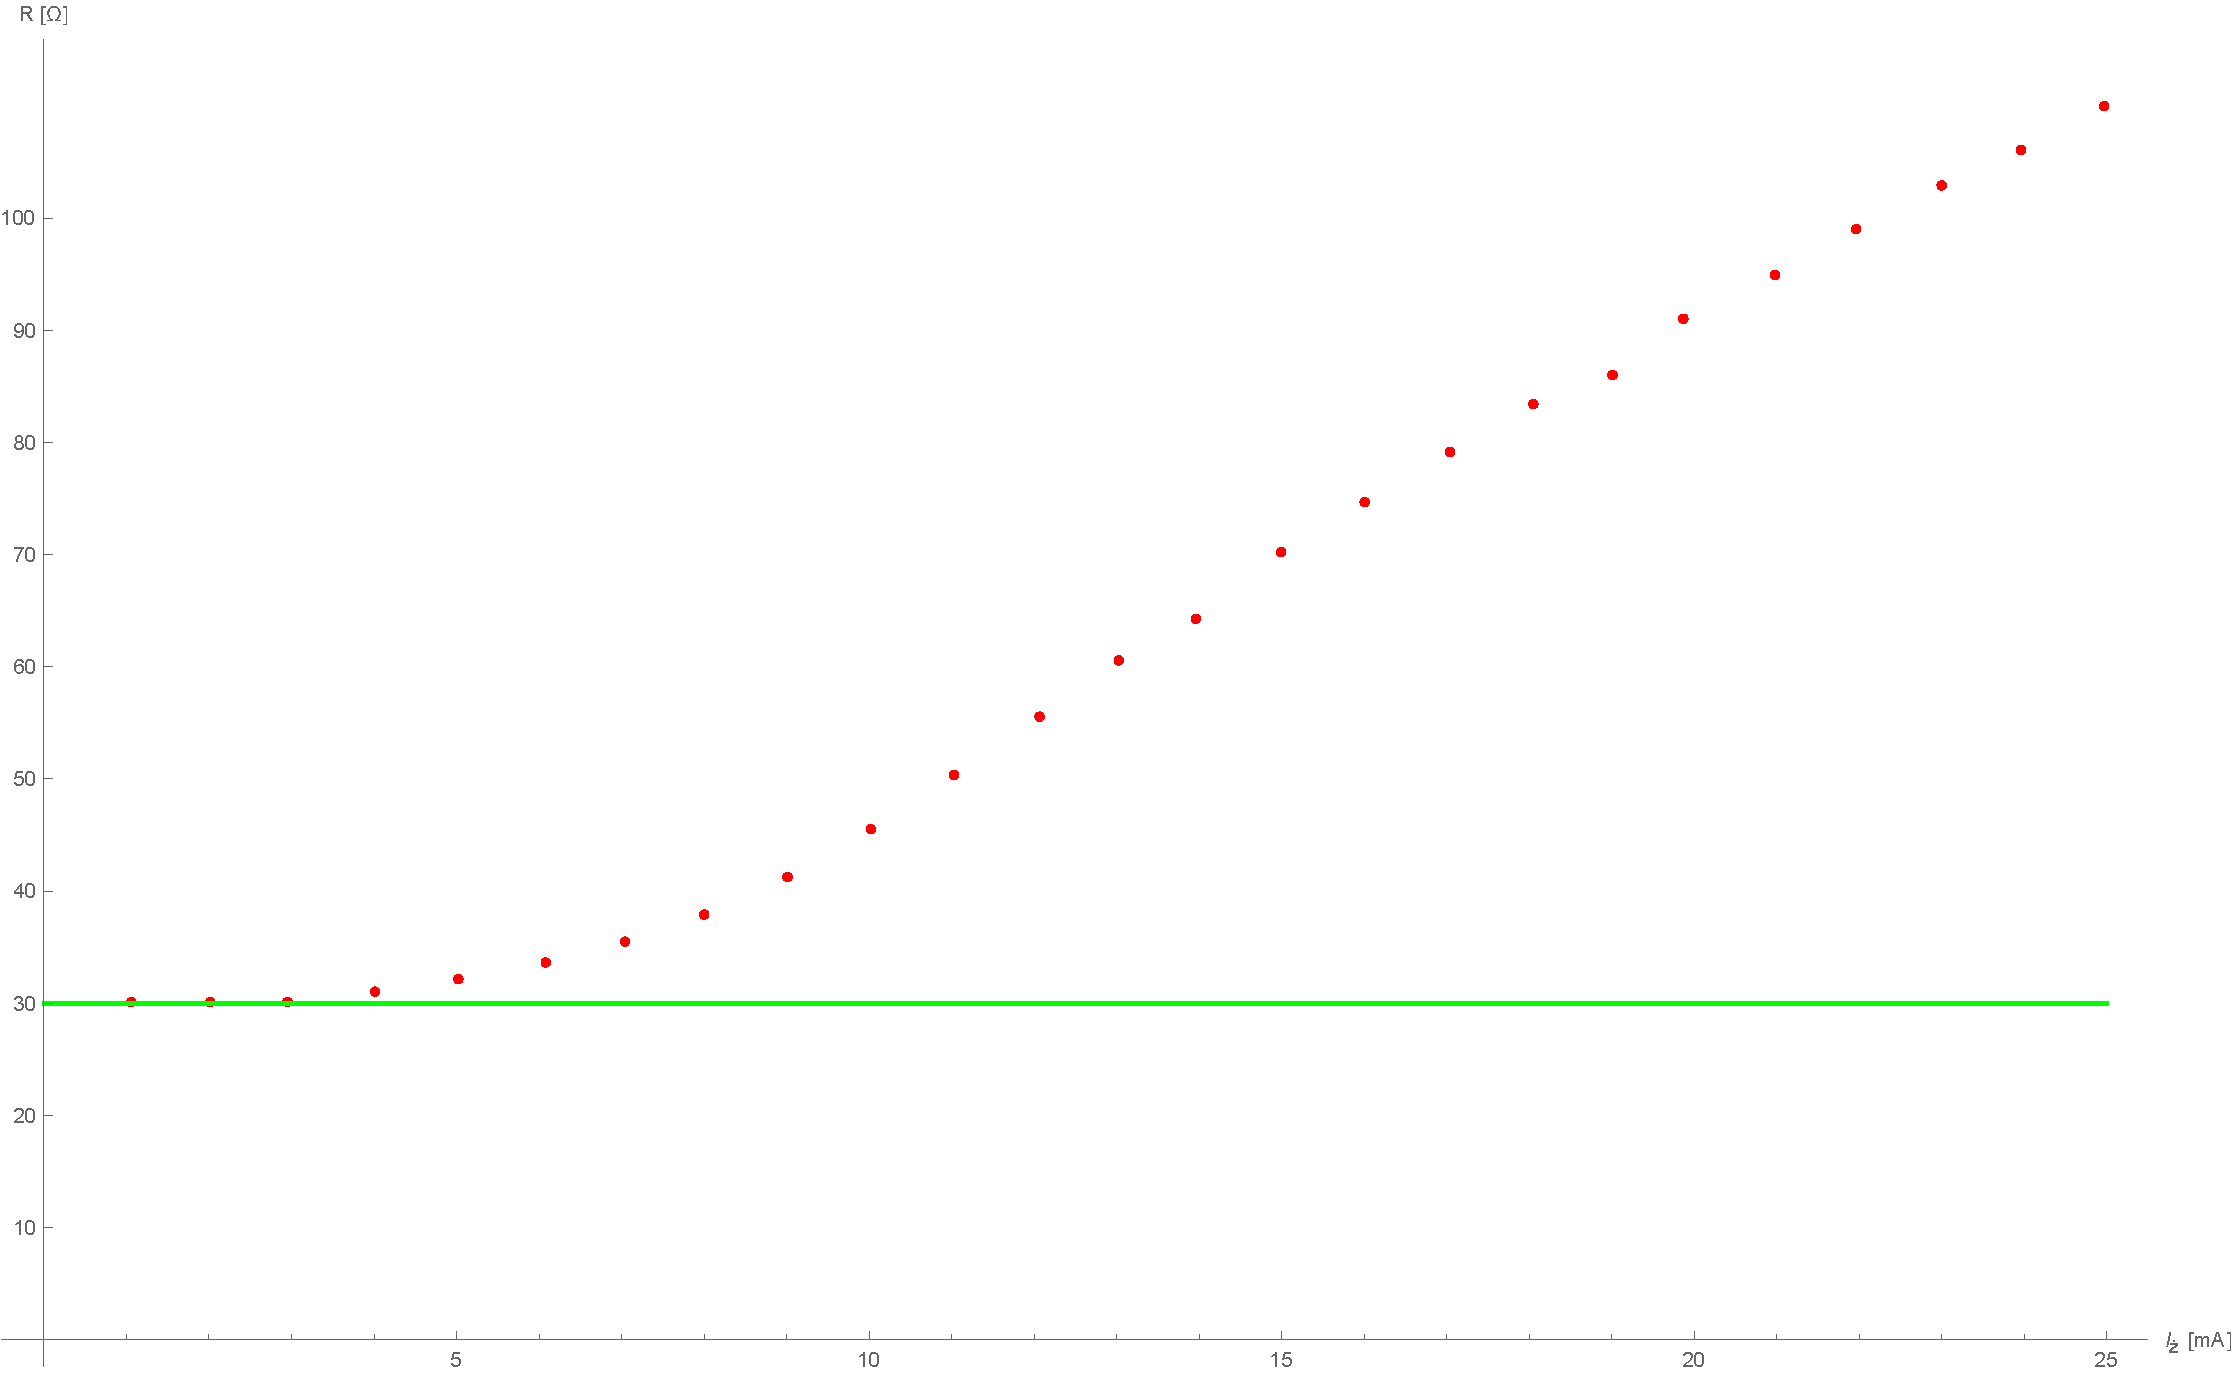
\includegraphics[width=0.9\linewidth]{rid}
\caption{Zależność oporu od prądu żarzenia. Możemy odczytać, że opór w temperaturze pokojowej wynosi $R_0=30\:\mathrm{\Omega}$.}
\label{fig:rid}
\end{figure}
Teraz możemy sprawdzić względną zmiannę rezystancji $\frac{R}{R_0}$. Z pomocą tabeli dołączonej do stanowiska pomiarowego zawierającej zależność względnej zmiany rezystancji od temperatury, możemy wyznaczyć funkcję $\frac{R}{R_0}=f(T)$:
\begin{figure}[h!]
\centering
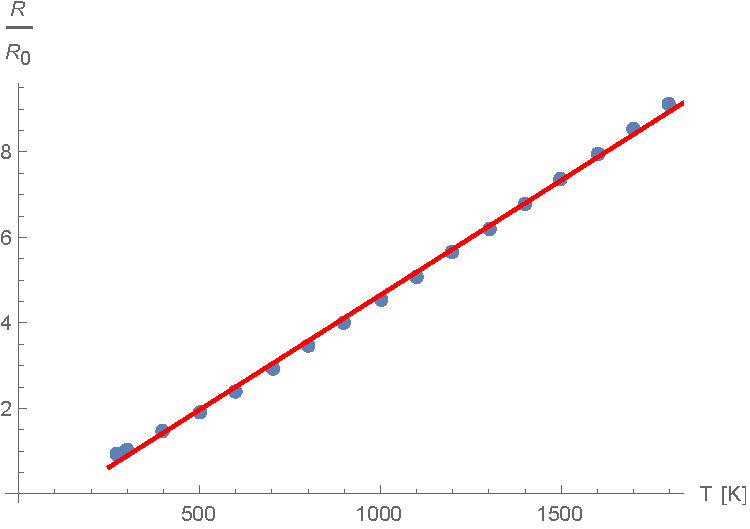
\includegraphics[width=0.6\linewidth]{temp}
\caption{Rezystancja względna jako funkcja temperatury. \newline
	Uzyskana postać to $\frac{R}{R_0}=0.00537016T-0.71812$.}
\label{fig:temp}
\end{figure}\clearpage

Mając temperaturę możemy już policzyć pracę wyjścia. Korzystamy ze wzoru:
\begin{align*}
W=\frac{2eI_\mathrm{ż}dI_\mathrm{ż}R}{I_a}-2k_b(T-T_0)
\end{align*}
Gdzie przyjęliśmy następujące wartości stałych i parametrów:
\begin{itemize}
	\item Stała Boltzmana $k_b=8.617\cdot10^{-5}\:\mathrm{\frac{eV}{K}}$
	\item Temperatura pokojowa $T_0=293.15\:\mathrm{K}$
	\item ładunek elementarny pozostawiliśmy jako jednostkę ładunku
\end{itemize}
W ten licząc dla pierwszych 11 pomiarów, gdzie prąd anodowy był wystarczająco duży, by można je brać pod uwagę(wyniki podane w $\mathrm{eV}$):
\begin{align*}
\begin{array}{|c|c|c|c|c|c|c|c|c|c|c|}
\hline
2.41478 & 2.24763 & 2.08107 & 1.92549 & 1.76181 & 1.59208 
 1.37419 & 1.28997 & 1.09604 & 1.20807 & 1.13367 \\ \hline
\end{array}
\end{align*}
\subsubsection{Wynik}
Licząc średnią dostajemy $W_{avg}=1.65\pm0.47\:\mathrm{eV}$. Gdzie niepewność policzyliśmy jako odchylenie standardowe.

\section{Wnioski}
\subsection{Metoda Richardsona}
Otrzymana wartość pracy wyjścia, to $W=4.95\pm0.22\:\mathrm{eV}$, a wartość tabelaryczna to $W_T=4.52\:\mathrm{eV}$.
Uzyskana przez nas wartość jest bliska wartości tabelarycznej, jednak znajduje się poza zakresem niepewności. Pomiary prowadzone były przy pomocy pirometru. Przyrząd ten wymaga doświadczenia, którego eksperymentatorowi brakowało. Jeśli weźmiemy pod uwagę niską dokładność pomiarów wynikajacą z tej przyczyny, to możemy uznać wynik za satysakcjonujący.
\subsection{Metoda Davissona}
Otrzymana przez nas wartość to $W=1.65\pm0.47\:\mathrm{eV}$. Wartość tabelaryczna to $W_T=1.5\:\mathrm{eV}$.
Widzimy, że wartość przez nas uzyskana jest bliska tablicowej, a jeśli weźmiemy pod uwagę drobne odchylenia związane ze zużyciem i możliwymi różnicami w budowie katody względem danych tablicowych, to możemy uznać tę wartość za wartość satysfakcjonującą.
\begin{thebibliography}{99}
	\bibitem{1} Ch. Kittel, \textit{Wstęp do Teorii ciała stałego}, PWN, Warszawa 1976 
	\bibitem{2} W. Gaponow, \textit{Elektronika}, t.2,  
	\bibitem{3} L. Kalinowski, \textit{Fizyka Metali}
\end{thebibliography}
\end{document}